\chapter{Appendix}
\section{M2M Transformational Rules from RUCM to Petri Net}\label{m2mrulesmain}


%\begin{figure}[H]
%  \centering
%    \subfloat[Rules for Initial State and Simple Basic Flow]{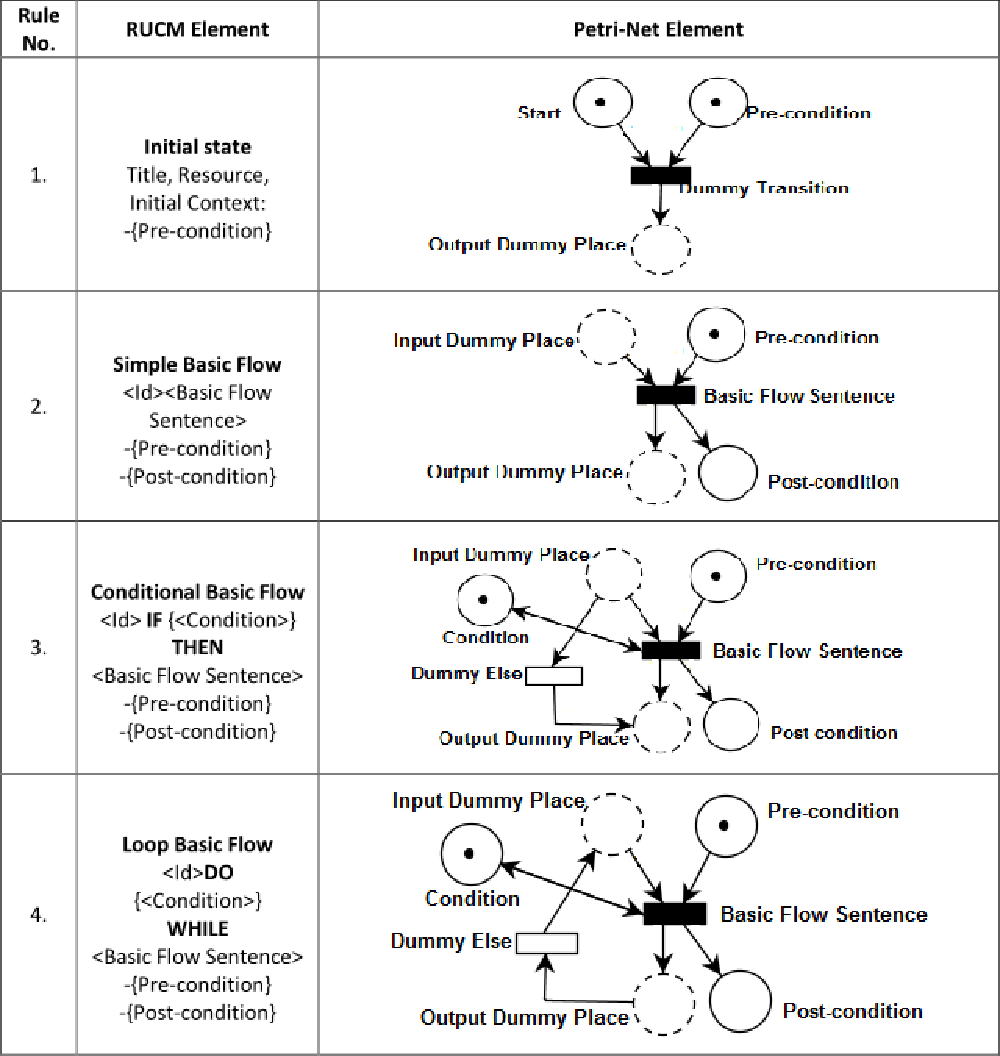
\includegraphics[width=0.6\textwidth,frame]{content/images/Appendix/fig1} \label{fig:rg_subfigAA}}
%    
%   \subfloat[Rules for Conditional Basic Flow and Loop Basic Flow]{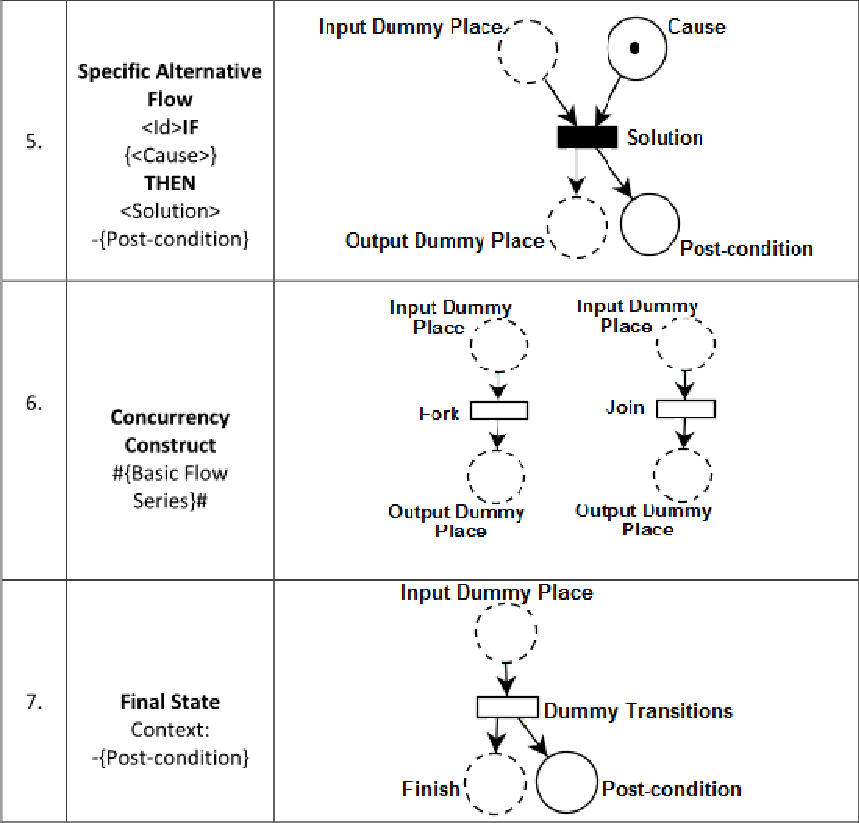
\includegraphics[width=0.6\textwidth,frame]{content/images/Appendix/fig2} \label{fig:rg_subfigBB}}
%   
%%     \subfloat[Rules for Specific Alternative Flow, Concurrency Construct and Final State]{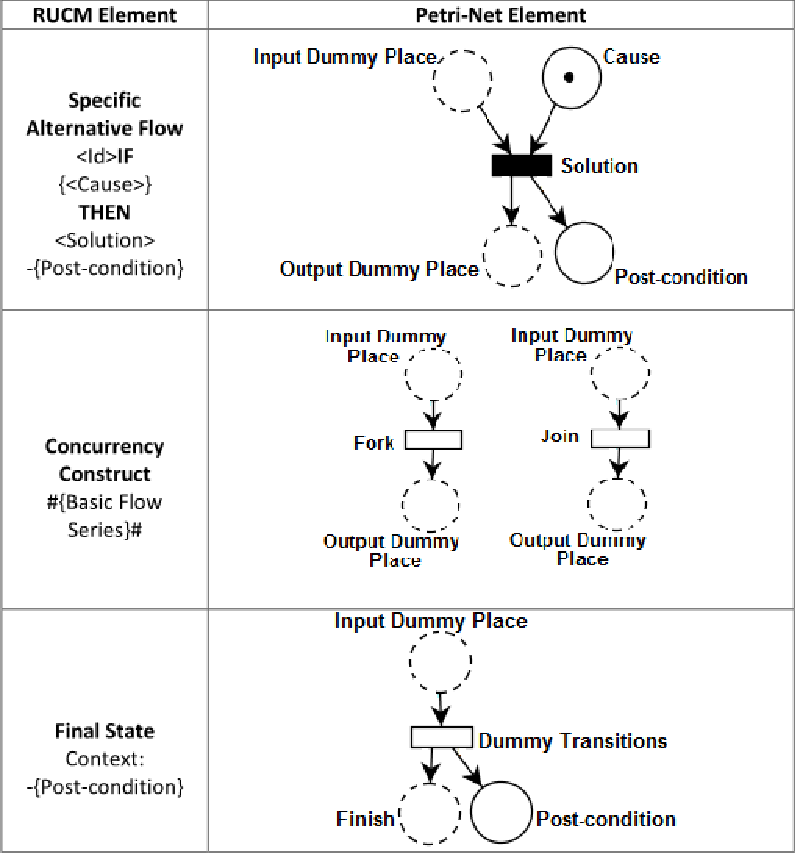
\includegraphics[width=0.6\textwidth,frame]{content/images/Appendix/fig3} \label{fig:rg_subfigCC}}
%	\caption{Concept of reachability.}
%\label{fig:rgconcept}
%\end{figure}

\begin{figure}[H]
\centering
\fbox{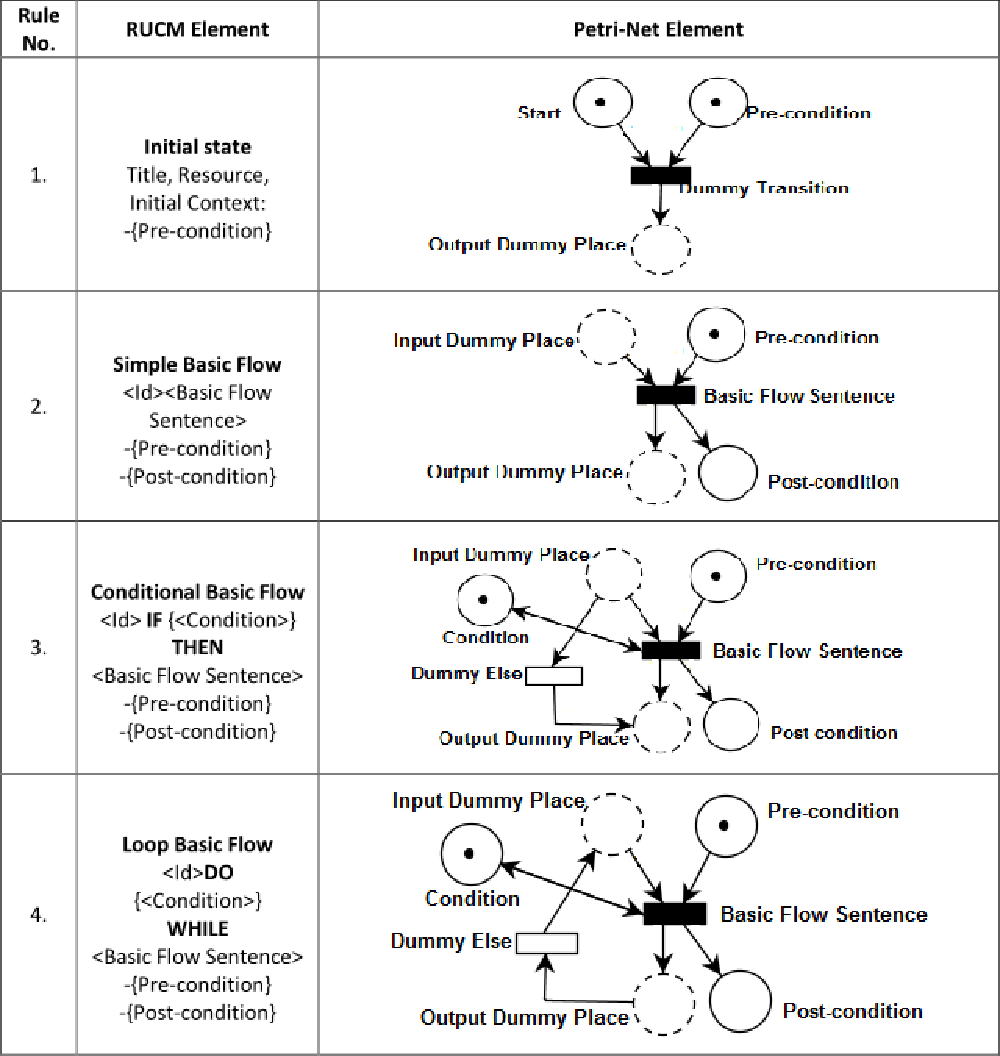
\includegraphics[width=0.55\textwidth]{content/images/Appendix/fig1}}
\caption{M2M Rules for Initial State and Simple Basic Flow}
\label{fig:m2mrulesdiagram1}
\end{figure}


\begin{figure}[H]
\centering
\fbox{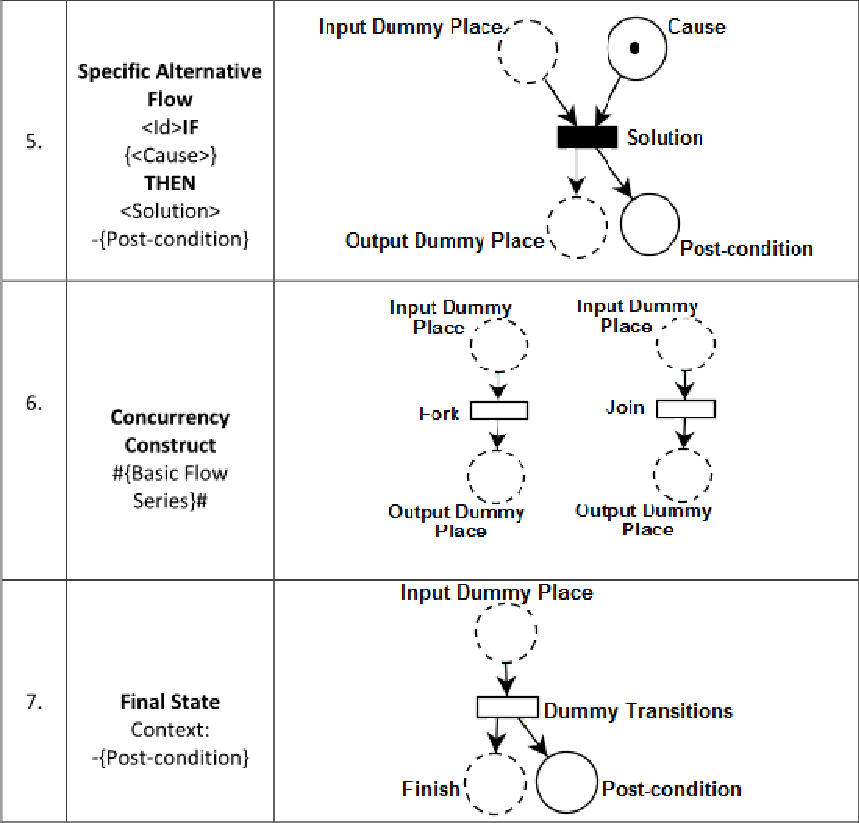
\includegraphics[width=0.55\textwidth]{content/images/Appendix/fig2}}
\caption{M2M Rules for Conditional Basic Flow and Loop Basic Flow}
\label{fig:m2mrulesdiagram2}
\end{figure}

\begin{figure}[H]
\centering
\fbox{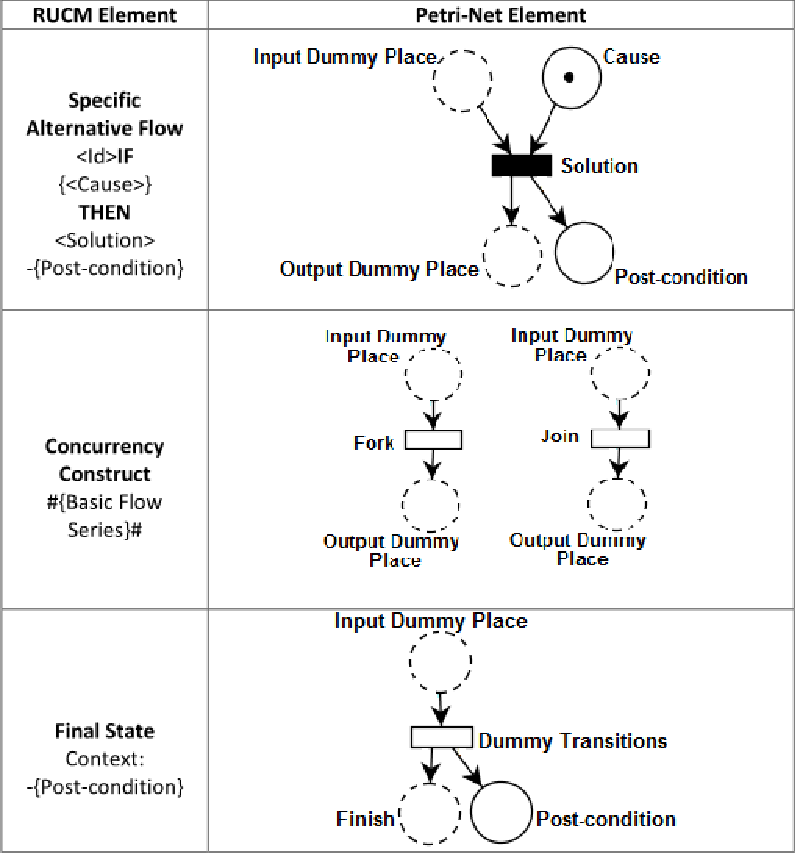
\includegraphics[width=0.55\textwidth]{content/images/Appendix/fig3}}
\caption{M2M Rules for Specific Alternative Flow, Concurrency and Final State}
\label{fig:m2mrulesdiagram3}
\end{figure}


\section{Implementation of M2M Transformational Rules for Sub Petri Nets to Integrated Petri Nets Conversion}\label{m2mrules}
\begin{minted}{qvto}
modeltype MMA uses "http://www.example.org/PetriNetMetaModel";
modeltype MMB uses "http://www.example.org/PetriNetMetaModel";

transformation PNtoPNTransformation(in Source: MMA, out Target: MMB);

main() {
	Source.rootObjects()[PetriNet] -> map PetriNetToPetriNet();
}

mapping PetriNet :: PetriNetToPetriNet() : PetriNet {
	/*This section makes calls to the different mappings 
	  required to integrate the sub Petri Nets*/
	result.place :=self.place -> map CopyOtherPlaceToNewPlace();
	result.place +=self.place -> map InputDummyPlaceToNewPlace();
	result.transition := self.transition -> map TransitionToNewTransition();
	
	result.arc := self.arc -> map InputArcToNewInputArc();
	result.arc += self.arc -> map InputArcToNewPlace();
	result.arc += self.arc -> map OutputArcToNewOutputArc();
	
	result.arc += self.arc -> map ExceptionInputArcToEpisodePlace();
	result.arc += self.arc -> map ConditionElseInputArcToEpisodePlace();
	result.arc += self.arc -> map ConditionElseOutputArcToEpisodePlace();
}

/*This following section contains the different mappings rules are 
		implemented according to their constraints*/
mapping Arc :: ConditionElseOutputArcToEpisodePlace() : Arc
when {self.Type.equalsIgnoreCase("Output") 
	and self.place.Name.startsWith("I_Dummy_Place")
	and self.transition.Name.equalsIgnoreCase("T_Dummy_Else") } {
   result.Weight := self.Weight;
   result.transition := self.transition
			.resolveoneIn(Transition :: TransitionToNewTransition, Transition);
   result.Type := self.Type;
      
   var var_Append: String;
   var_Append:= self.place.Name.at(15);
   var var_Next:Integer;
   var_Next:= var_Append.toInteger()+1;
   
   var temp : Place;
   temp := self.place.container().allSubobjectsOfType(Place)
		->any(Name.toString().startsWith("I_Dummy_Place_"+var_Append));
   result.place := temp.resolveoneIn( Place :: InputDummyPlaceToNewPlace, Place);
}

mapping Arc :: ConditionElseInputArcToEpisodePlace() : Arc
when {self.Type.equalsIgnoreCase("Input") 
	and self.place.Name.startsWith("O_Dummy_Place")
	and self.transition.Name.equalsIgnoreCase("T_Dummy_Else") } {
   result.Weight := self.Weight;
   result.transition := self.transition
			.resolveoneIn(Transition :: TransitionToNewTransition, Transition);
   result.Type := self.Type;
     
   var var_Append: String;
   var_Append:= self.place.Name.at(15);
   var var_Next:Integer;
   var_Next:= var_Append.toInteger()+1;
   
   var temp : Place;
   temp := self.place.container().allSubobjectsOfType(Place)
		->any(Name.toString().startsWith("I_Dummy_Place_"+var_Next.toString()));
   result.place := temp.resolveoneIn( Place :: InputDummyPlaceToNewPlace, Place);
 }

mapping Arc :: ExceptionInputArcToEpisodePlace() : Arc
when {self.Type.equalsIgnoreCase("Input") 
	and self.place.Name.startsWith("I_E_Dummy") } {
   result.Weight := self.Weight;
   result.transition := self.transition
			.resolveoneIn(Transition :: TransitionToNewTransition, Transition);
   result.Type := self.Type;
      
   var var_Append: Integer;
   var_Append:= self.place.Name.at(11).toInteger()+1;
   var temp : Place;   
   var var_Count:Integer;
   var var_Set:Collection(Place);
   var_Set:= self.place.container().allSubobjectsOfType(Place)
		->select(Name.toString().startsWith("I_Dummy_Place_"));
   var_Count := var_Set->size();
   
   var var_Next:Integer;
   var_Next:= var_Append;
	
	if(var_Next = var_Count)then{
	temp := self.place.container().allSubobjectsOfType(Place)
		->any(Name.toString().startsWith("I_Dummy_Place_E"));
	result.place := temp.resolveoneIn( Place :: InputDummyPlaceToNewPlace, Place);
	}else{
	temp := self.place.container().allSubobjectsOfType(Place)
		->any(Name.toString().startsWith("I_Dummy_Place_"+var_Append.toString()));   
	result.place := temp.resolveoneIn( Place :: InputDummyPlaceToNewPlace, Place);
	}endif;  
}
	
mapping Arc :: OutputArcToNewOutputArc() : Arc
when {self.Type.equalsIgnoreCase("Output") 
	and  self.place.Name.startsWith("O_Dummy_Place") } {
   result.Weight := self.Weight;
   result.transition := self.transition
			.resolveoneIn(Transition :: TransitionToNewTransition, Transition);
   result.Type := self.Type;  
   
    var var_Count:Integer;
    var var_Set:Collection(Place);
    var_Set:= self.place.container().allSubobjectsOfType(Place)
			->select(Name.toString().startsWith("I_Dummy_Place_"));
    var_Count := var_Set->size();
  
    var var_Append: String;
    var_Append:= self.place.Name.at(15);
	if(var_Append.equalsIgnoreCase("S"))then{
	var_Append := 1.toString();
	var temp : Place;
	temp := self.place.container().allSubobjectsOfType(Place)
		->any(Name.toString()
		.startsWith("I_Dummy_Place_"+var_Append.toString()));
	result.place := temp.resolveoneIn(Place :: InputDummyPlaceToNewPlace, Place);
	}else{
	var var_Next:Integer;
	var_Next:= var_Append.toInteger()+1;
	var temp : Place;
   
	if(var_Next = var_Count)then{
	temp := self.place.container().allSubobjectsOfType(Place)
		->any(Name.toString().startsWith("I_Dummy_Place_E"));
	result.place := temp.resolveoneIn( Place :: InputDummyPlaceToNewPlace, Place);
	}else{   
	temp := self.place.container().allSubobjectsOfType(Place)
		->any(Name.toString().startsWith("I_Dummy_Place_"+var_Next.toString()));
	result.place := temp.resolveoneIn( Place :: InputDummyPlaceToNewPlace, Place);
	}endif;
	}endif;     
}

mapping Arc :: InputArcToNewPlace() : Arc
when {(self.Type.equalsIgnoreCase("Input") 
	and self.place.Name.startsWith("I_Dummy_Place"))} {
   result.Weight := self.Weight;
   result.transition := self.transition
			.resolveoneIn(Transition :: TransitionToNewTransition, Transition);
   result.place := self.place.resolveoneIn( Place :: InputDummyPlaceToNewPlace, Place);
   result.Type := self.Type;      
}

mapping Arc :: InputArcToNewInputArc() : Arc
when {(self.Type.equalsIgnoreCase("Input") 
	and not self.place.Name.startsWith("I_Dummy_Place") 
	and not self.place.Name.startsWith("I_E_Dummy") 
	and not self.place.Name.startsWith("O_Dummy_Place")) 
	or (self.Type.equalsIgnoreCase("Output") 
	and not (self.place.Name.startsWith("O_Dummy_Place")
	or self.place.Name.startsWith("I_Dummy_Place")))} {
   result.Weight := self.Weight;
   result.transition := self.transition
			.resolveoneIn(Transition :: TransitionToNewTransition, Transition);
   result.place := self.place.resolveoneIn(Place :: CopyOtherPlaceToNewPlace, Place);
   result.Type := self.Type;      
}

mapping Transition :: TransitionToNewTransition() : Transition {
   result.Name:=self.Name;         
}	
	
mapping Place :: InputDummyPlaceToNewPlace() : Place
when {self.Name.startsWith("I_Dummy_Place")} {
   result.Tokens:=self.Tokens;
   result.Name:=  "P" + self.Name.toString().at(15);      
}

mapping Place :: CopyOtherPlaceToNewPlace() : Place 
when {not (self.Name.startsWith("O_Dummy_Place")
 	or self.Name.startsWith("I_Dummy_Place")
 	or self.Name.startsWith("I_E_Dummy") )}{
   result.Tokens:=self.Tokens;
   result.Name:=  self.Name;     
}			
\end{minted}


\section{Implementation of M2T Transformational Rules for Petri Net to PNML Conversion}\label{m2trules} 
\begin{minted}{xtend}

«IMPORT PetriNetMetaModel»

/*To create net details in the corresponding tag in PNML*/
«DEFINE main FOR PetriNet»
«FILE "IntegratedPetriNet.xml"»<?xml version="1.0" encoding="ISO-8859-1"?><pnml>
<net id="Net-One" type="P/T net">
<token id="Default" enabled="true" red="0" green="0" blue="0"/>
«EXPAND placedetails FOREACH place»
«EXPAND transdetails FOREACH transition»
«EXPAND arcdetails FOREACH arc»</net>
</pnml>
«ENDFILE»	
«ENDDEFINE»

/*To create the place details in the corresponding tag in PNML*/
«DEFINE placedetails FOR Place»<place id="«this.Name»">
<name>
<value>«this.Name»</value>
</name>
<initialMarking>
<value>Default,«this.Tokens»</value>
</initialMarking>
<capacity>
<value>«this.Tokens»</value>
</capacity>
</place>
«ENDDEFINE»

/*To create transition details in the corresponding tag in PNML*/
«DEFINE transdetails FOR Transition»<transition id="«this.Name»">
<name>
<value>«this.Name»</value>
</name>
<rate>
<value>1.0</value>
</rate>
<timed>
<value>«if this.Name.contains("T_Dummy_End") then "true" else "false"»</value>
</timed>
<infiniteServer>
<value>false</value>
</infiniteServer>
<priority>
<value>1</value>
</priority>
</transition>
«ENDDEFINE»


/*To create arc details in the corresponding tag in PNML*/
«DEFINE arcdetails FOR Arc»<arc id="
«if this.Type.contains("Input") then this.place.Name else this.transition.Name» to 
«if this.Type =="Input" then this.transition.Name else this.place.Name»" source="
«if this.Type =="Input" then this.place.Name else this.transition.Name»" target="
«if this.Type =="Input" then this.transition.Name else this.place.Name»">
<inscription>
<value>Default,1</value>
</inscription>
<tagged>
<value>false</value>
</tagged>
<type value="normal"/>
</arc>
«ENDDEFINE»
\end{minted}
